% latex cheat sheet for spatial data handling in R - modify to suit AniMove.org needs
% based on cheatsheets latex document of J. Stein, T. Short and E. Paradis

\documentclass[10pt,landscape]{article}
\usepackage{multicol}
\usepackage{calc}
\usepackage{ifthen}
\usepackage[landscape]{geometry}
\usepackage{graphicx}
\usepackage{hyperref}

\hypersetup{
  colorlinks, linkcolor=blue, urlcolor=blue
}


% To make this come out properly in landscape mode, do one of the following
% 1.
%  pdflatex latexsheet.tex
%
% 2.
%  latex latexsheet.tex
%  dvips -P pdf  -t landscape latexsheet.dvi
%  ps2pdf latexsheet.ps


% If using another size paper, use default 1cm margins.
\ifthenelse{\lengthtest { \paperwidth = 11in}}
	{ \geometry{top=.5in,left=.5in,right=.5in,bottom=.5in} }
	{\ifthenelse{ \lengthtest{ \paperwidth = 297mm}}
		{\geometry{top=1cm,left=1cm,right=1cm,bottom=1cm} }
		{\geometry{top=1cm,left=1cm,right=1cm,bottom=1cm} }
	}

% Turn off header and footer
\pagestyle{empty}
 

% Redefine section commands to use less space
\makeatletter
\renewcommand{\section}{\@startsection{section}{1}{0mm}%
                                {-1ex plus -.5ex minus -.2ex}%
                                {0.5ex plus .2ex}%x
                                {\normalfont\large\bfseries}}
\renewcommand{\subsection}{\@startsection{subsection}{2}{0mm}%
                                {-1explus -.5ex minus -.2ex}%
                                {0.5ex plus .2ex}%
                                {\normalfont\normalsize\bfseries}}
\renewcommand{\subsubsection}{\@startsection{subsubsection}{3}{0mm}%
                                {-1ex plus -.5ex minus -.2ex}%
                                {1ex plus .2ex}%
                                {\normalfont\small\bfseries}}
\makeatother

% Define BibTeX command
\def\BibTeX{{\rm B\kern-.05em{\sc i\kern-.025em b}\kern-.08em
    T\kern-.1667em\lower.7ex\hbox{E}\kern-.125emX}}

% Don't print section numbers
\setcounter{secnumdepth}{0}


\setlength{\parindent}{0pt}
\setlength{\parskip}{0pt plus 0.5ex}

\usepackage[nodayofweek]{datetime}

% -----------------------------------------------------------------------

\begin{document}

\newlength{\MyLen}
\settowidth{\MyLen}{\texttt{letterpaper}/\texttt{a4paper} \ }


\raggedright
\footnotesize
\begin{multicols}{3}


% multicol parameters
% These lengths are set only within the two main columns
%\setlength{\columnseprule}{0.25pt}
\setlength{\premulticols}{1pt}
\setlength{\postmulticols}{1pt}
\setlength{\multicolsep}{1pt}
\setlength{\columnsep}{2pt}

\begin{center}
     \Large{\textbf{AniMove Cheat Sheet}} \\
     for spatial data handling, remote sensing, spatial statistics and animal movement analysis
\end{center}

\begin{center}
 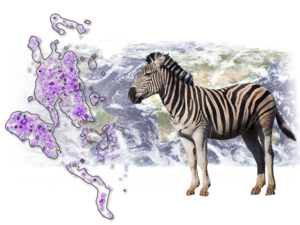
\includegraphics[width=.22\textwidth]{pics/animove_org_WegmannBevanda_zebra_africa_dbb_light.png}
 % rhino.png: 719x1056 pixel, 300dpi, 6.09x8.94 cm, bb=0 0 173 253
\end{center}


\url{www.animove.org}\\
last updated: \today

\rule{0.32\textwidth}{0.4pt}


\section{Packages}
\begin{tabular}{@{}ll@{}}
\verb!raster!    & for raster data manipulation \\
\verb!sp!     & for vector data manipulation \\
\verb!rgdal!  & data import and export, projections \\
\verb!rgeos!  & geometry commands \\
\verb!spdep!  & spatial dependence \\
\verb!dismo!  &  species distribution modelling \\
\verb!move!  & access and analyse movement data\\
\verb!bcpa!  & analyse movement tracks\\
& \\
further relevant packages:\\
% 
\verb!spatstat!  & spatial statistics\\
\verb!gstat!  & geostatistics\\
\verb!geoR!  & geostatistical analysis\\
\verb!gdistance!  & distances on geographical grids\\
\verb!spsurvey!  & sampling functionality\\
\verb!trip!  & sp class extension for track analysis\\
\verb!randomForest!  & random Forest implementation\\
\verb!mgcv!  & GAM implementation\\
\verb!lme4!  & mixed-effects model\\
\verb!landsat!  & Landsat specific analysis\\
\verb!spgrass6!  & interaction with GRASS\\
% 
& \\
visualisation packages:\\
\verb!maptools!  & handling spatial objects\\
\verb!maps!  & map display\\
\verb!mapproj!  & map projections\\
\verb!mapdata!  & supplements to maps\\
\verb!rasterVis!  & enhanced raster visualisation\\
\verb!ggplot2!  & for more fancy plots\\
\verb!reshape2!  & flexibly reshape data \\
 & 
\end{tabular}

More spatial R packages are listed here: cran.r-project.org/web/views/Spatial.html

\rule{0.32\textwidth}{0.4pt}
Relevant commands are listed below, actual syntax needs to be checked within the manual pages of each command. 
\rule{0.32\textwidth}{0.4pt}



\section{\textbf{Raster}}

Raster data manipulation is similar to a spreadsheet or matrix manipulation but with coordinates and projections, hence various also not explictly spatial commands can be applied. Here we  mainly list commands designed for spatial data handling.

\subsubsection{Import and export}

\begin{tabular}{@{}p{\the\MyLen}%
                @{}p{\linewidth-\the\MyLen}@{}}
                
raster() & import (or generate) one raster layer \\
brick() & import raster with multiple layers \\
writeRaster()   & export raster data to file\\
writeFormats() & list of supported raster file types \\
getData() & retrieves DEM and climate data directly from the web
\end{tabular}


\subsubsection{Information}

\begin{tabular}{@{}p{\the\MyLen}%
                @{}p{\linewidth-\the\MyLen}@{}}
print()   & prints raster metadata   \\     
click()   & interactively query raster plot \\
hist()    & histogram of raster values per layer \\
cellStats()  & summary statistics of single layers \\
summary() & summary statistics \\
extent()  & extent of raster data set \\
ncell()   & number of cells (of one layer)\\
nlayers() & number of bands \\
names() & prints layer names \\
str()	& print the data structure \\
NAvalue() & get or set background values

\end{tabular}


\subsubsection{Visualisation}

\begin{tabular}{@{}p{\the\MyLen}%
                @{}p{\linewidth-\the\MyLen}@{}}
plot(), plotRGB()  & raster plot and RGB plot. Usefull arguments: y=bandnumber, add=TRUE (overlay multiple plots)  \\
image(), spplot() & alternative plotting commands\\
levelplot() & fancy way to plot raster data information \\
densityplot() & raster value density plot \\
bwplot() & violin plot of raster data values \\
hovmoller() & spatio-temporal plotting options \\
streamplot() & plotting of streamlines

\end{tabular}







\subsubsection{Projections}

\begin{tabular}{@{}p{\the\MyLen}%
                @{}p{\linewidth-\the\MyLen}@{}}
projection()	  & query or set projection (does NOT reproject)\\                
projectRaster()   & reprojects raster to new coordinate system \\

\end{tabular}


\subsubsection{Data manipulation}
Most raster commands will output a file to a chosen location, if filename= is specified. Otherwise it will use temp files.

\begin{tabular}{@{}p{\the\MyLen}%
                @{}p{\linewidth-\the\MyLen}@{}}
 &  \\                
stack() & stack different raster layers together \\
addLayer(); dropLayer()	& add/drop a raster layer\\
crop() 		& crop raster set to smaller extent  \\
drawExtent()	& draw extent on a plot for e.g. inclusion in crop(raster,extent)\\
mask() 		& masking of background values \\
merge(); mosaic() & combine raster tiles to a raster with larger extent \\
extract() 	& extract values from Raster objects, using points or polygons  \\
raster*2/raster2 & any basic operation, more efficient: \\                
calc()  	& apply a function to raster data and\\
overlay()       & apply a function which uses multiple bands, e.g. to calculate NDVI \\
focal()         & moving window operations \\
distance()      & calculate distance to closest feature, e.g. distance to water\\
terrain() 	& calculate terrain attributes from DEM, e.g. slope \\
zonal()         & zonal statistics, for classified raster\\
reclassify()	& reclassify raster values \\
subs()		& substitutes values \\
resample() 	& resampling of raster to raster \\
aggregate()	& aggregation of cells \\
disaggregate()	& disaggregation of cells \\
rasterToPoints() & converts a raster to vector points	\\
rasterToPolygons() & converts a raster to polygons \\
rasterToContour()  & converts raster values to contour \\
$[[$\ $]]$		& address specific raster layer, e.g. myRaster[[1]] for first layer of myRaster    \\  
x $<$- raster $>$ 50	& boolean operation, output is binary \\
raster[raster $<=$ 50] $<$- 0 & replace all values smaller then 50 with 0 \\
r1[r1$==$50] $<$- r2[r1$==$50] & values in r1 whose values are equal 50 are replaced by the corresponding values of r2 \\
		&			 \\
  sampleRandom() & random sample from cell values\\
  sampleRegular() & regular sample from cell values\\
  sampleStratified() & stratified sample from cell values\\
  
\end{tabular}



\rule{0.32\textwidth}{0.4pt}


\section{\textbf{Vector}}

Vector data often come in shp format including a variety of auxiliary files. All of them are relevant and are needed for further analysis. Note that readShapePoly() etc. from package maptools do 
NOT automatically read projection information from shapefiles. It is reccomended to use readOGR() instead.

\subsubsection{Import and export}

\begin{tabular}{@{}p{\the\MyLen}%
                @{}p{\linewidth-\the\MyLen}@{}}
                
readOGR() 		& import vector file \\
writeOGR() 		& export vector file \\
ogrDrivers() 	& list supported file formats \\


\end{tabular}

\subsubsection{Information}

\begin{tabular}{@{}p{\the\MyLen}%
                @{}p{\linewidth-\the\MyLen}@{}}

                plot()  & vector plot. add=TRUE overlays multiple plots, e.g. combine with raster data  \\
summary() & metadata and data summary \\                
extent() & extent/bounding box of vector data \\
coordinates()	& sets spatial coordinates to create spatial data, or retrieves spatial coordinates\\

\end{tabular}


\subsubsection{Projections}

\begin{tabular}{@{}p{\the\MyLen}%
                @{}p{\linewidth-\the\MyLen}@{}}
                
projection()	  & query or set projection (does NOT reproject)\\                               
spTransform()	  & reproject vector data to new coordinate system \\
               

\end{tabular}


\subsubsection{Data manipulation}

Check out the functions in the rgeos package, which provides most of the classical vector GIS operations such as buffers etc.\\


\begin{tabular}{@{}p{\the\MyLen}%
                @{}p{\linewidth-\the\MyLen}@{}}
                & \\
subset()		& subset spatial data, based on a condition, e.g. keep only certain points \\                
merge() 		& Merge a Spatial object having a data.frame (i.e. merging of non-spatial attributes)\\
over()			& spatial overlay for points, grids and polygons \\
rasterize() 		& Rasterize points, lines, or polygons\\ 
distanceFromPoints()    & computes the distance to points, output is a raster\\
extract()		& extracts raster values behind points, lines or polygons \\
gIntersection()		& intersection of vector data sets \\
gBuffer()		& Buffer Geometry \\
 & 
\end{tabular}


\rule{0.32\textwidth}{0.4pt}



\section{Spatial Modeling}

\begin{tabular}{@{}p{\the\MyLen}%
                @{}p{\linewidth-\the\MyLen}@{}}
kfold() & partitioning of data set for training/validation purpose\\
evaluate() & cross-validation of models with presence/absence data\\               
randomForest() & fits a randomForest model  \\
maxent() & executes Maxent from R\\
gam() & fits a GAM \\
pls() & fits a partial least squares model \\                
predict() & predicts statistical model into space (raster) \\

 & 

\end{tabular}


\rule{0.32\textwidth}{0.4pt}
\scriptsize


\section{Movement Analysis}

For most of the following commands the data sets need to be converted to a specific format.


\begin{tabular}{@{}p{\the\MyLen}%
                @{}p{\linewidth-\the\MyLen}@{}}
                & \\
move() & import of movement data sets from movebank.org  \\
moveStack() & stacks multiple animal tracks \\
split() & splits stack into single move objects \\
movebankLogin() & stores movebank.org credentials \\
searchMovebankStudies() & reports the studies in movebank.org matching search criteria\\
getMovebankData() & import tracks directly from movebank.org \\
show() & summary of the move object \\
as() & coerce movement between object types \\
angle() &  extracts turning angles from a move object\\\newdateformat{mydate}{\twodigit{\THEDAY}{ }\shortmonthname[\THEMONTH], \THEYEAR}
speed() & extracts speed from a move object \\  
distance() & extracts distance between locations from a move object \\
time.lag() & extracts time lag between locations from a move object \\
spTransform() & changes the projection of a move object to a default of Azimuthal Equi-distance \\
mcp() & calculates minimum convex polygons for SpPdf \\
kernelUD() & calculates a kernel density surface for SpPdf \\
brownian.bridge() & claculates constant variance Brownian bridges \\
brownian.bridge.dyn() & calculates dynamic Brownian bridges \\
LoCoH.k() & calculates local convex hulls using k neighbours \\
LoCoH.r() & calculates local convex hulls using a radius of r \\
LoCoH.a() & calculates local convex hulls using an adpative radius \\
% .. & ... \\
& 

\end{tabular}


%\rule{0.32\textwidth}{0.4pt}


\section{Miscellaneous}

Some useful commands which are related to spatial data analysis.


\begin{tabular}{@{}p{\the\MyLen}%
                @{}p{\linewidth-\the\MyLen}@{}}
                & \\
gmap() & get google maps for your plot \\
geocode() & geocoding in R \\
ggplot() & lots of very fancy plotting options \\
ppp() & creates a point pattern \\
%show() & summary of the move object \\

complete.cases() &  returns only cases with no missing values \\                
gridSample() & sample point from a grid e.g. just one point per pixel \\

 & \\
function(...)\{..\} & generates a defined functions\\
return(...) & returns the output of a function \\
if (...) \{...\} else\{...\} & if else statement \\
for (...) \{...\} & for loop \\
while (...) \{ ...\} & while statement \\
 & \\


\end{tabular}



% \rule{0.3\linewidth}{0.25pt}

\scriptsize

\rule{0.32\textwidth}{0.4pt}

compiled by: Wegmann, Leutner, Bevanda, Horning \& Safi \\ \THEYEAR	

\url{http://www.animove.org}


\bigskip

\bigskip

% \begin{center}
%  \includegraphics[width=.3\textwidth]{../../Pictures/webpage/animove/rhino.png}
%  % zebra_crop_ppt.png: 1006x872 pixel, 72dpi, 35.49x30.76 cm, bb=0 0 1006 872
% \end{center}


\begin{center}
 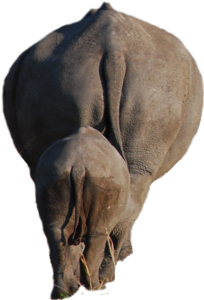
\includegraphics[width=.2\textwidth]{pics/earth-observation_org_WegmannBevanda_rhino_family.png}
 % rhino.png: 719x1056 pixel, 300dpi, 6.09x8.94 cm, bb=0 0 173 253
\end{center}



\end{multicols}
\end{document}
